\section{Data}

\subsection{FairFace}
The FairFace dataset contains 108,501 face
images collected primarily from the YFCC-100M Flickr dataset. Attributes include age, gender, and race, and is notably balanced in distribution across the seven racial/ethnic groups represented in the dataset (White, Black, Indian, East Asian, Southeast Asian,
Middle East, and Latino)  \cite{krkkinen2019fairface}. There are no names or ids in the dataset, so it cannot be used to judge how accurately a facial recognition model can identify a person based on an image.
\begin{center} 
Five images from the FairFace training dataset.
\\
{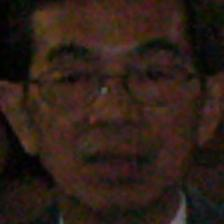
\includegraphics[width=0.18\textwidth]{figure/fairface_1.jpg}}
{
\includegraphics[width=0.18\textwidth]{figure/fairface_2.jpg}}
{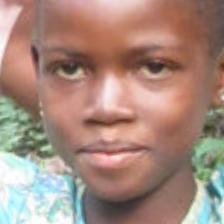
\includegraphics[width=0.18\textwidth]{figure/fairface_3.jpg}}
{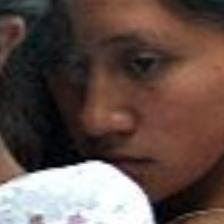
\includegraphics[width=0.18\textwidth]{figure/fairface_4.jpg}}
{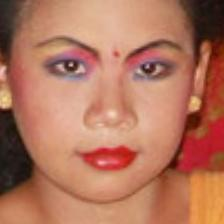
\includegraphics[width=0.18\textwidth]{figure/fairface_5.jpg}}
\end{center}
\begin{table}[H]
\centering
\caption{Attributes of the above images.}
\begin{tabular}{lllll}
file & age & gender & race \\
train/1.jpg & 50-59 & Male & East Asian \\
train/2.jpg & 30-39 & Female & Indian\\
train/3.jpg & 3-9 & Female & Black  \\
train/4.jpg & 20-29 & Female & Indian\\
train/5.jpg & 20-29 & Female & Indian        
\end{tabular}
\end{table}

\subsection{IMDb-Faces} \label{imdb_data}
The IMDb-Faces dataset contains 460,723 face images from 20,284 celebrities from IMDb. Attributes include gender, birthdate, name, and year when the photo was taken \cite{Rothe-ICCVW-2015}. Notably, there is no information on race or ethnicity, which poses an issue for algorithm fairness: many face recognition models are unfair with respect to race/ethnicity because there is significant class imbalance in the dataset. More specifically, there are often many more white subjects in the dataset than subjects of other races/ethnicities — which is true of the IMDb-Faces dataset \cite{shepley2019deep}. Because we do not have label information for race or ethnicity, we cannot correct this imbalance. Furthermore, since we do not have ethnicity information, we cannot use it as a feature in our training or testing. 
\\
\\
As a solution, we webscraped ethnicity information for celebrities from ethniccelebs.com, and cleaned these longer ethnic data into one of the seven ethnic categories from FairFace. Our cleaned IMDb dataset, with ethnicity, contains 347,701 face images from 6,224 celebrities.

\begin{center}
Five images from the IMDb-Faces dataset.\\
{
\includegraphics[width=0.18\textwidth]{figure/imdb_1.jpg}}
{
\includegraphics[width=0.18\textwidth]{figure/imdb_2.jpg}}
{
\includegraphics[width=0.18\textwidth]{figure/imdb_3.jpg}}
{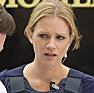
\includegraphics[width=0.18\textwidth]{figure/imdb_4.jpg}}
{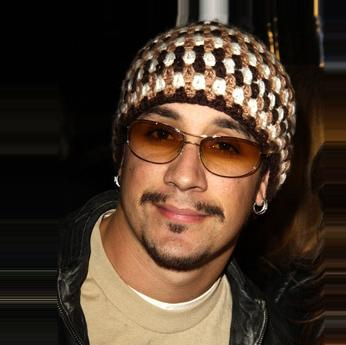
\includegraphics[width=0.18\textwidth]{figure/imdb_5.jpg}}
\end{center}
\begin{table}[H]
\small
\centering
\caption{Cleaned attributes of the above images.}
\begin{tabular}{llllll}
celeb\_id & name &  gender & ethnicity & full\_path \\
2 & Weird Al Yankovic & Male & White & Weird\_Al\_Yankovic\_0.jpg \\
4 & 50 Cent & Male & Black & 50\_Cent\_0.jpg \\
5 & A Martinez & Male & Latino & A\_Martinez\_0.jpg  \\
8 & A.J. Cook & Female & White & A.J.\_Cook\_0.jpg \\
11 & A.J. McLean & Male & Latino & A.J.\_McLean\_0.jpg \\
\end{tabular}
\end{table}
\noindent Interestingly, two of the faces (1 and 2) clearly do not match the celebrity name label. Likely, these are costars of the labelled celebrity whose faces were also tagged in their IMDb images. However, it raises the issue of inaccuracies in the dataset.